


%%% outline
%-------------------------------------------------------------------------


%%% 简易机器翻译系统 - step 3 decoding - example


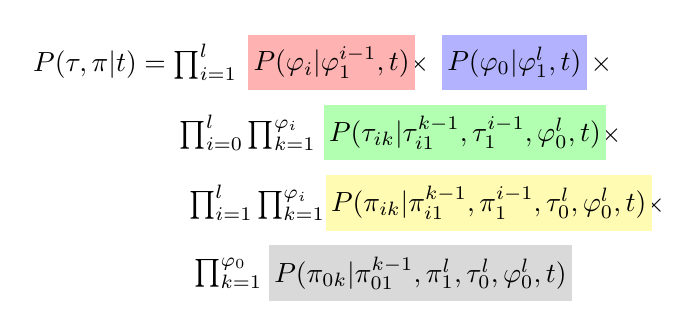
\begin{tikzpicture}



\node [anchor=west,inner sep=2pt,minimum height=2.5em] (eq1) at (0,0) {${\funp{P}(\tau,\pi|\seq{t}) =  \prod_{i=1}^{l}\hspace{6.0em} \times \ \hspace{5.5em}\times}$};
\node [anchor=north west,inner sep=2pt,minimum height=2.5em] (eq2) at ([xshift=-16.06em,yshift=0.0em]eq1.south east) {${\prod_{i=0}^l{\prod_{k=1}^{\varphi_i}\hspace{9.6em}} \ \ \times}$};
\node [anchor=north west,inner sep=2pt,minimum height=2.5em] (eq3) at ([xshift=-16.05em,yshift=0.0em]eq2.south east) {${\prod_{i=1}^l{\prod_{k=1}^{\varphi_i}}\hspace{11.5em} \times}$};
\node [anchor=north west,inner sep=2pt,minimum height=2.5em] (eq4) at ([xshift=-17.44em,yshift=0.0em]eq3.south east) {{${\prod_{k=1}^{\varphi_0}}$}};

\node [anchor=west,inner sep=2pt,minimum height=2.0em,fill=red!30] (part1) at ([xshift=-13.4em,yshift=0.0em]eq1.east) {{${\funp{P}(\varphi_i|\varphi_{1}^{i-1},\seq{t})}$}};
\node [anchor=west,inner sep=2pt,minimum height=2.0em,fill=blue!30] (part2) at ([xshift=-6.4em,yshift=0.0em]eq1.east) {{${\funp{P}(\varphi_0|\varphi_{1}^{l},\seq{t})}$}};
\node [anchor=west,inner sep=2pt,minimum height=2.0em,fill=green!30] (part3) at ([xshift=-11em,yshift=0.0em]eq2.east) {{${\funp{P}(\tau_{ik}|\tau_{i1}^{k-1},\tau_{1}^{i-1},\varphi_{0}^{l},\seq{t} )}$}};
\node [anchor=west,inner sep=2pt,minimum height=2.0em,fill=yellow!30] (part4) at ([xshift=-12.5em,yshift=0.0em]eq3.east) {{${\funp{P}(\pi_{ik}|\pi_{i1}^{k-1},\pi_{1}^{i-1},\tau_{0}^{l},\varphi_{0}^{l},\seq{t} )}$}};
\node [anchor=west,inner sep=2pt,minimum height=2.0em,fill=gray!30] (part5) at ([xshift=0.0em,yshift=0.0em]eq4.east) {{${\funp{P}(\pi_{0k}|\pi_{01}^{k-1},\pi_{1}^{l},\tau_{0}^{l},\varphi_{0}^{l},\seq{t} )}$}};


\end{tikzpicture}



































